\subsubsection{2.2. Kết quả kiểm thử trên các mô hình CNN baseline}
\indent\indent Dưới đây là kết quả kiểm thử chi tiết của sáu mô hình CNN baseline, trong đó các giá trị được lấy từ lần chạy đạt kết quả cao nhất.\vspace{0.3cm}

\textbf{* ResNet18}
\begin{table}[H]
\centering
\renewcommand{\arraystretch}{1.0}
\caption{Classification report của ResNet18 trên CNN baseline}
\label{tab:CRResNet18}
\begin{tabular}{lcccc}
\hline
\textbf{Lớp} & \textbf{Precision} & \textbf{Recall} & \textbf{F1-Score} & \textbf{Support} \\
\hline
cho-noi-cai-rang          & 0.9333 & 0.9333 & 0.9333 & 45 \\
dua-bo-bay-nui             & 0.9574 & 1.0000 & 0.9783 & 45 \\
hoi-lim                    & 0.9333 & 0.9333 & 0.9333 & 45 \\
le-hoi-nghinh-ong          & 0.8108 & 0.6667 & 0.7317 & 45 \\
nghe-dan-tre               & 0.9565 & 0.9778 & 0.9670 & 45 \\
nghe-det-chieu             & 0.9318 & 0.9111 & 0.9213 & 45 \\
ok-om-bok                  & 0.9762 & 0.9111 & 0.9425 & 45 \\
via-ba-chua-xu-nui-sam     & 0.7037 & 0.8444 & 0.7677 & 45 \\
\hline
\textbf{Accuracy}          & & & 0.8972 & 360 \\
\textbf{Macro avg}         & 0.9004 & 0.8972 & 0.8969 & 360 \\
\textbf{Weighted avg}      & 0.9004 & 0.8972 & 0.8969 & 360 \\
\hline
\end{tabular}
\end{table}
%===================================================================
\newpage
\textbf{* RegNetX400MF}
\begin{table}[H]
\centering
\renewcommand{\arraystretch}{1.0}
\caption{Classification report của RegNetX400MF trên CNN baseline}
\label{tab:CRRegNetX400MF}
\begin{tabular}{lcccc}
\hline
\textbf{Lớp} & \textbf{Precision} & \textbf{Recall} & \textbf{F1-Score} & \textbf{Support} \\
\hline
cho-noi-cai-rang          & 0.8958 & 0.9556 & 0.9247 & 45 \\
dua-bo-bay-nui             & 0.9783 & 1.0000 & 0.9890 & 45 \\
hoi-lim                    & 0.8077 & 0.9333 & 0.8660 & 45 \\
le-hoi-nghinh-ong          & 0.8000 & 0.6222 & 0.7000 & 45 \\
nghe-dan-tre               & 0.9565 & 0.9778 & 0.9670 & 45 \\
nghe-det-chieu             & 0.9744 & 0.8444 & 0.9048 & 45 \\
ok-om-bok                  & 1.0000 & 0.9111 & 0.9535 & 45 \\
via-ba-chua-xu-nui-sam     & 0.6792 & 0.8000 & 0.7347 & 45 \\
\hline
\textbf{Accuracy}          & & & 0.8806 & 360 \\
\textbf{Macro avg}         & 0.8865 & 0.8806 & 0.8800 & 360 \\
\textbf{Weighted avg}      & 0.8865 & 0.8806 & 0.8800 & 360 \\
\hline
\end{tabular}
\end{table}
%===================================================================
\textbf{* MobileNetV3 Large}
\begin{table}[H]
\centering
\renewcommand{\arraystretch}{1.0}
\caption{Classification report của MobileNetV3 Large trên CNN baseline}
\label{tab:CRMobileNetV3Large}
\begin{tabular}{lcccc}
\hline
\textbf{Lớp} & \textbf{Precision} & \textbf{Recall} & \textbf{F1-Score} & \textbf{Support} \\
\hline
cho-noi-cai-rang          & 0.9565 & 0.9778 & 0.9670 & 45 \\
dua-bo-bay-nui             & 0.9783 & 1.0000 & 0.9890 & 45 \\
hoi-lim                    & 0.8958 & 0.9556 & 0.9247 & 45 \\
le-hoi-nghinh-ong          & 0.8750 & 0.6222 & 0.7273 & 45 \\
nghe-dan-tre               & 0.9348 & 0.9556 & 0.9451 & 45 \\
nghe-det-chieu             & 0.9302 & 0.8889 & 0.9091 & 45 \\
ok-om-bok                  & 0.9773 & 0.9556 & 0.9663 & 45 \\
via-ba-chua-xu-nui-sam     & 0.7091 & 0.8667 & 0.7800 & 45 \\
\hline
\textbf{Accuracy}          & & & 0.9028 & 360 \\
\textbf{Macro avg}         & 0.9071 & 0.9028 & 0.9011 & 360 \\
\textbf{Weighted avg}      & 0.9071 & 0.9028 & 0.9011 & 360 \\
\hline
\end{tabular}
\end{table}
%===================================================================
\textbf{* MobileNetV3 Small}
\begin{table}[H]
\centering
\renewcommand{\arraystretch}{1.0}
\caption{Classification report của MobileNetV3 Small trên CNN baseline}
\label{tab:CRMobileNetV3Small}
\begin{tabular}{lcccc}
\hline
\textbf{Lớp} & \textbf{Precision} & \textbf{Recall} & \textbf{F1-Score} & \textbf{Support} \\
\hline
cho-noi-cai-rang          & 0.9184 & 1.0000 & 0.9574 & 45 \\
dua-bo-bay-nui            & 0.9778 & 0.9778 & 0.9778 & 45 \\
hoi-lim                   & 0.7925 & 0.9333 & 0.8571 & 45 \\
le-hoi-nghinh-ong         & 0.8636 & 0.4222 & 0.5672 & 45 \\
nghe-dan-tre              & 0.9111 & 0.9111 & 0.9111 & 45 \\
nghe-det-chieu            & 0.9070 & 0.8667 & 0.8864 & 45 \\
ok-om-bok                 & 0.9286 & 0.8667 & 0.8966 & 45 \\
via-ba-chua-xu-nui-sam    & 0.5902 & 0.8000 & 0.6792 & 45 \\
\hline
\textbf{Accuracy}         &        &        & 0.8472 & 360 \\
\textbf{Macro avg}        & 0.8611 & 0.8472 & 0.8416 & 360 \\
\textbf{Weighted avg}     & 0.8611 & 0.8472 & 0.8416 & 360 \\
\hline
\end{tabular}
\end{table}
%===================================================================
\newpage
\textbf{* DenseNet121}
\begin{table}[H]
\centering
\renewcommand{\arraystretch}{1.0}
\caption{Classification report khi kiểm thử DenseNet121 trên CNN baseline}
\label{tab:CRDenseNet121}
\begin{tabular}{lcccc}
\hline
\textbf{Lớp} & \textbf{Precision} & \textbf{Recall} & \textbf{F1-Score} & \textbf{Support} \\
\hline
cho-noi-cai-rang          & 0.9565 & 0.9778 & 0.9670 & 45 \\
dua-bo-bay-nui             & 0.9783 & 1.0000 & 0.9890 & 45 \\
hoi-lim                    & 0.9348 & 0.9556 & 0.9451 & 45 \\
le-hoi-nghinh-ong          & 0.7857 & 0.7333 & 0.7586 & 45 \\
nghe-dan-tre               & 0.9767 & 0.9333 & 0.9545 & 45 \\
nghe-det-chieu             & 0.9318 & 0.9111 & 0.9213 & 45 \\
ok-om-bok                  & 0.9348 & 0.9556 & 0.9451 & 45 \\
via-ba-chua-xu-nui-sam     & 0.7447 & 0.7778 & 0.7609 & 45 \\
\hline
\textbf{Accuracy}          & & & 0.9056 & 360 \\
\textbf{Macro avg}         & 0.9054 & 0.9056 & 0.9052 & 360 \\
\textbf{Weighted avg}      & 0.9054 & 0.9056 & 0.9052 & 360 \\
\hline
\end{tabular}
\end{table}
%===================================================================
\textbf{* ShuffleNetV2 1.0x}
\begin{table}[H]
\centering
\renewcommand{\arraystretch}{1.0}
\caption{Classification report khi kiểm thử ShuffleNet V2 1.0x trên CNN baseline}
\label{tab:CRShuffleNetV2X1.0}
\begin{tabular}{lcccc}
\hline
\textbf{Lớp} & \textbf{Precision} & \textbf{Recall} & \textbf{F1-Score} & \textbf{Support} \\
\hline
cho-noi-cai-rang          & 0.8696 & 0.8889 & 0.8791 & 45 \\
dua-bo-bay-nui             & 0.9149 & 0.9556 & 0.9348 & 45 \\
hoi-lim                    & 0.7925 & 0.9333 & 0.8571 & 45 \\
le-hoi-nghinh-ong          & 0.6667 & 0.4444 & 0.5333 & 45 \\
nghe-dan-tre               & 0.9767 & 0.9333 & 0.9545 & 45 \\
nghe-det-chieu             & 0.8889 & 0.8889 & 0.8889 & 45 \\
ok-om-bok                  & 0.9697 & 0.7111 & 0.8205 & 45 \\
via-ba-chua-xu-nui-sam     & 0.5873 & 0.8222 & 0.6852 & 45 \\
\hline
\textbf{Accuracy}          & & & 0.8222 & 360 \\
\textbf{Macro avg}         & 0.8333 & 0.8222 & 0.8192 & 360 \\
\textbf{Weighted avg}      & 0.8333 & 0.8222 & 0.8192 & 360 \\
\hline
\end{tabular}
\end{table}

\indent Dựa trên kết quả kiểm thử chi tiết của các mô hình CNN baseline, tôi rút ra những nhận xét sau:\vspace{-0.1cm}
\begin{itemize}[label={--}, itemsep=1pt]
    \item Về khả năng trích xuất đặc trưng của kiến trúc mạng:\vspace{-0.1cm}
    \begin{itemize}[label={+}, itemsep=1pt]
        \item \textbf{Nhóm mô hình nặng (DenseNet121, ResNet18):} DenseNet121 đạt kết quả cao nhất (0.9056), cho thấy cơ chế kết nối dày đặc (dense connectivity) giúp bảo toàn thông tin cực tốt khi lan truyền qua các lớp, cho phép mô hình nắm bắt tốt được các đặc trưng của dữ liệu ảnh ICH.
        \item \textbf{Nhóm mô hình nhẹ (MobileNet, RegNet, ShuffleNet):} Có sự bất ngờ lớn ở MobileNetV3 Large, dù là kiến trúc hướng di động, nhưng độ chính xác đạt được vẫn rất cao (0.9028), tiệm cận DenseNet121 và vượt qua cả ResNet18. Điều này chứng tỏ các khối \textit{Inverted Residuals} và cơ chế \textit{Squeeze-and-Excitation} của nó hoạt động rất hiệu quả trên tập dữ liệu này. Ngược lại, khi giảm số lượng tham số xuống quá thấp như ở MobileNetV3 Small hay ShuffleNetV2 1.0x, khả năng biểu diễn của mô hình bị suy giảm đáng kể (giảm khoảng 6\%-8\% so với nhóm dẫn đầu).
    \end{itemize}
    \newpage
    \item Về độ khó phân loại giữa các lớp:\vspace{-0.1cm}
    \begin{itemize}[label={+}, itemsep=1pt]
        \item \textbf{Các lớp có đặc trưng hình ảnh mạnh:} Lớp \textit{dua-bo-bay-nui} luôn đạt F1-Score trên 0.97 ở hầu hết các mô hình, có thể lý giải rằng các khung cảnh về "ruộng bùn" và "cặp bò đang chạy" là những đặc trưng độc nhất, ít bị trùng lặp với các lớp khác, giúp mô hình dễ dàng phân loại chính xác ngay cả với kiến trúc yếu như ShuffleNet.
        \item \textbf{Sự nhập nhằng ngữ nghĩa:} Lớp \textit{le-hoi-nghinh-ong} là thách thức lớn nhất, với F1-Score thấp kỷ lục (chỉ 0.53 ở ShuffleNet và khoảng 0.75 ở DenseNet). Việc Recall của lớp này thường xuyên ở mức thấp cho thấy mô hình bỏ sót rất nhiều mẫu thực tế. Nguyên nhân có thể do sự tương đồng về bối cảnh sông nước, tàu thuyền với lớp \textit{cho-noi-cai-rang}, khiến mô hình chỉ dựa vào hình ảnh đơn thuần rất khó phân biệt rạch ròi.
    \end{itemize}
\end{itemize}

%===================================================================
Dưới đây là bảng tổng hợp và biểu đồ thể hiện kết quả trung bình của tất cả 6 mô hình CNN baseline:
\begin{table}[H]
\centering
\caption{Kết quả kiểm thử trung bình của tất cả các mô hình CNN baseline}
\label{tab:CNNBaselineSummary}
\renewcommand{\arraystretch}{1.15}
\begin{tabular}{lcccc}
\hline
\textbf{Mô hình} & \textbf{Accuracy} & \textbf{Precision} & \textbf{Recall} & \textbf{F1-Score} \\
\hline
ResNet18              & 0.8907 & 0.8936 & 0.8907 & 0.8905 \\
RegNetX400MF          & 0.8806 & 0.8860 & 0.8806 & 0.8797 \\
MobileNetV3 Large     & \textbf{0.9028} & \textbf{0.9076} & \textbf{0.9028} & \textbf{0.9006} \\
MobileNetV3 Small     & 0.8379 & 0.8547 & 0.8379 & 0.8329 \\
DenseNet121           & 0.8963 & 0.8976 & 0.8963 & 0.8955 \\
ShuffleNetV2 1.0x     & 0.8204 & 0.8314 & 0.8204 & 0.8172 \\
\hline
\end{tabular}
\end{table}

\begin{figure}[H]
    \centering
    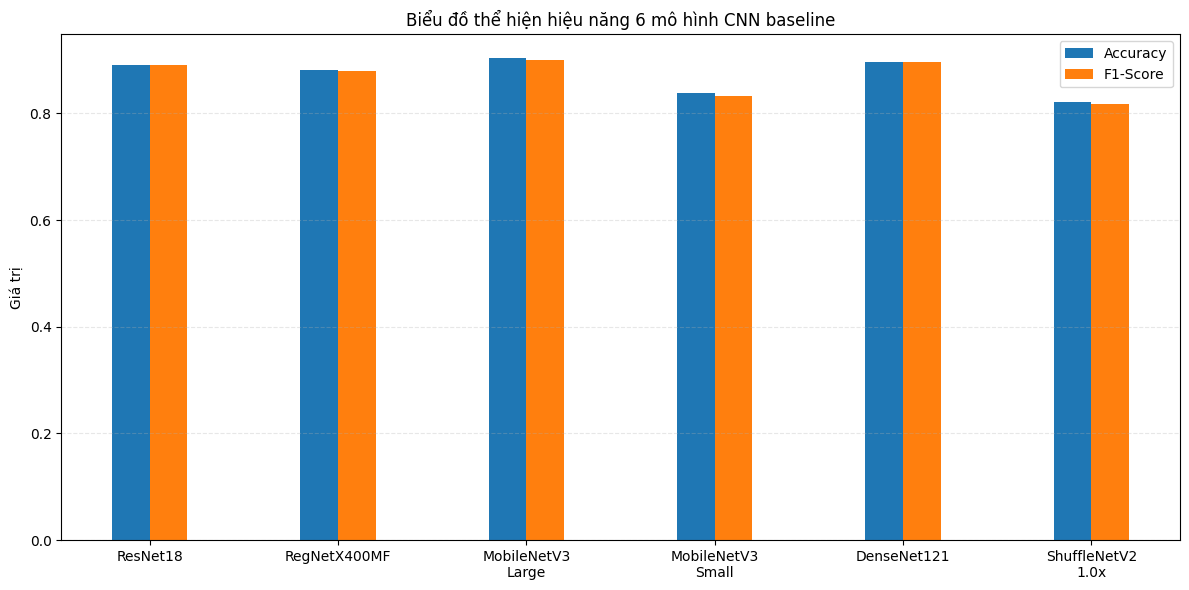
\includegraphics[width=\linewidth]{images/part-02/chap-03/sec-02/CNNBaseline.png}
    \caption{Biểu đồ thể hiện hiệu năng của 6 mô hình CNN baseline}
    \label{fig:CNNBaseline}
\end{figure}

\indent Dựa trên bảng tổng hợp và biểu đồ thể hiện kết quả trung bình của 6 mô hình CNN baseline, tôi đưa ra các kết luận sau:\vspace{-0.1cm}
\begin{itemize}[label={--}, itemsep=1pt]
    \item MobileNetV3 Large đã cho thấy tính vượt trội trong bài toán này khi đạt kết quả cao nhất trên toàn bộ các thang đo (Accuracy: 0.9028, F1-Score: 0.9006). Mặc dù là một kiến trúc được thiết kế tối ưu cho thiết bị di động với số lượng tham số ít hơn nhiều so với ResNet18 hay DenseNet121, nhưng cơ chế \textit{Hard-Swish} và cấu trúc \textit{Inverted Residual} đặc biệt của nó dường như rất phù hợp để trích xuất các đặc trưng văn hóa trong tập dữ liệu này. 

    \item DenseNet121, ResNet18 và RegNetX400MF cũng cho ra độ chính xác rất sát lần lượt là 0.8963, 0.8907 và 0.8806 . Dù DenseNet có kết quả đơn lẻ cao nhất (như đã phân tích ở phần trước), nhưng khi xét trung bình, nó kém hơn MobileNetV3 Large một khoảng nhỏ. Điều này cho thấy các mô hình nặng vẫn hoạt động tốt nhưng chưa chắc đã là lựa chọn tối ưu nhất về mặt cân bằng giữa hiệu suất và chi phí tính toán cho bài toán cụ thể này.

    \item Hai mô hình MobileNetV3 Small và ShuffleNetV2 1.0x cho thấy sự sụt giảm hiệu năng đáng kể (lần lượt là 0.8379 và 0.8204). Mức chênh lệch lên tới gần 8\% so với nhóm dẫn đầu cho thấy việc nén mô hình quá mức đã làm mất đi khả năng phân biệt các chi tiết phức tạp trong các lễ hội có bối cảnh tương đồng.
\end{itemize}

Kết quả kiểm thử cho thấy phương pháp CNN baseline (chỉ sử dụng hình ảnh) có thể đạt ngưỡng chính xác khoảng \textbf{0.9}. Tuy nhiên, việc không thể vượt qua ngưỡng này cùng với những hạn chế trong việc phân loại các lớp nhập nhằng (như đã phân tích ở lớp \textit{le-hoi-nghinh-ong}) đặt ra nhu cầu cấp thiết phải bổ sung thêm thông tin từ 2 phương thức khác là văn bản và âm thanh.